% !TeX root = main.tex
\subsection{Airfoil Selection and sizing}

The design happens in the following stages

\subsubsection*{Specifications}

We assume a takeoff weight of $2\,kg$. The environment temperature is assumed to be $25^\circ C$, where density of air is $\rho = 1.184\,kg/m^3$ an the dynamic viscosity is $\mu = 1.849 \times 10^{-5} kg/(ms)$ \footnote{Values obtained from \url{https://lynniezulu.com/what-is-the-dynamic-viscosity-of-air/}}. For now, the cruise speed can be $20\,m/s$.

For the starting, we will assume the wing to be rectangular and with chord length $c = \bar{c} = 0.2\,m$. Let us also assume the wingspan be to $b = 1.1\,m$. These are values taken from the UAVs in the market survey.

\subsubsection*{Wing Design - Phase 1: Airfoil analysis}

We will choose \texttt{NACA 2412} airfoil for starting the design phase (simply because it is common for remote controlled UAVs). It is shown in figure \ref{fig:naca-2412-prof}.


\begin{figure}[ht]
    \centering
    \begin{subfigure}[b]{0.45\textwidth}
        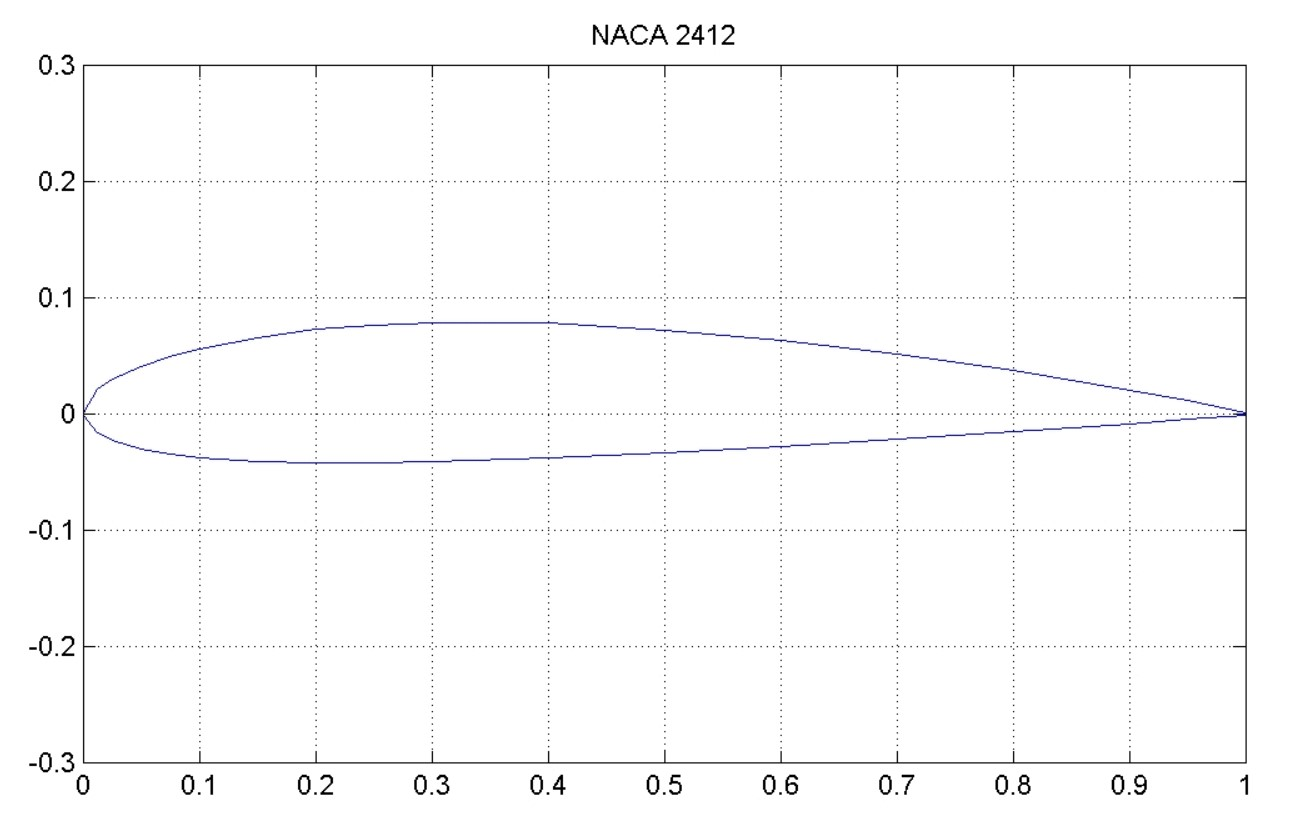
\includegraphics[width=\textwidth]{naca-2412-profile.jpg}
        \caption{NACA-2412 Profile}
        \label{fig:naca-2412-prof}
    \end{subfigure}
    \begin{subfigure}[b]{0.45\textwidth}
        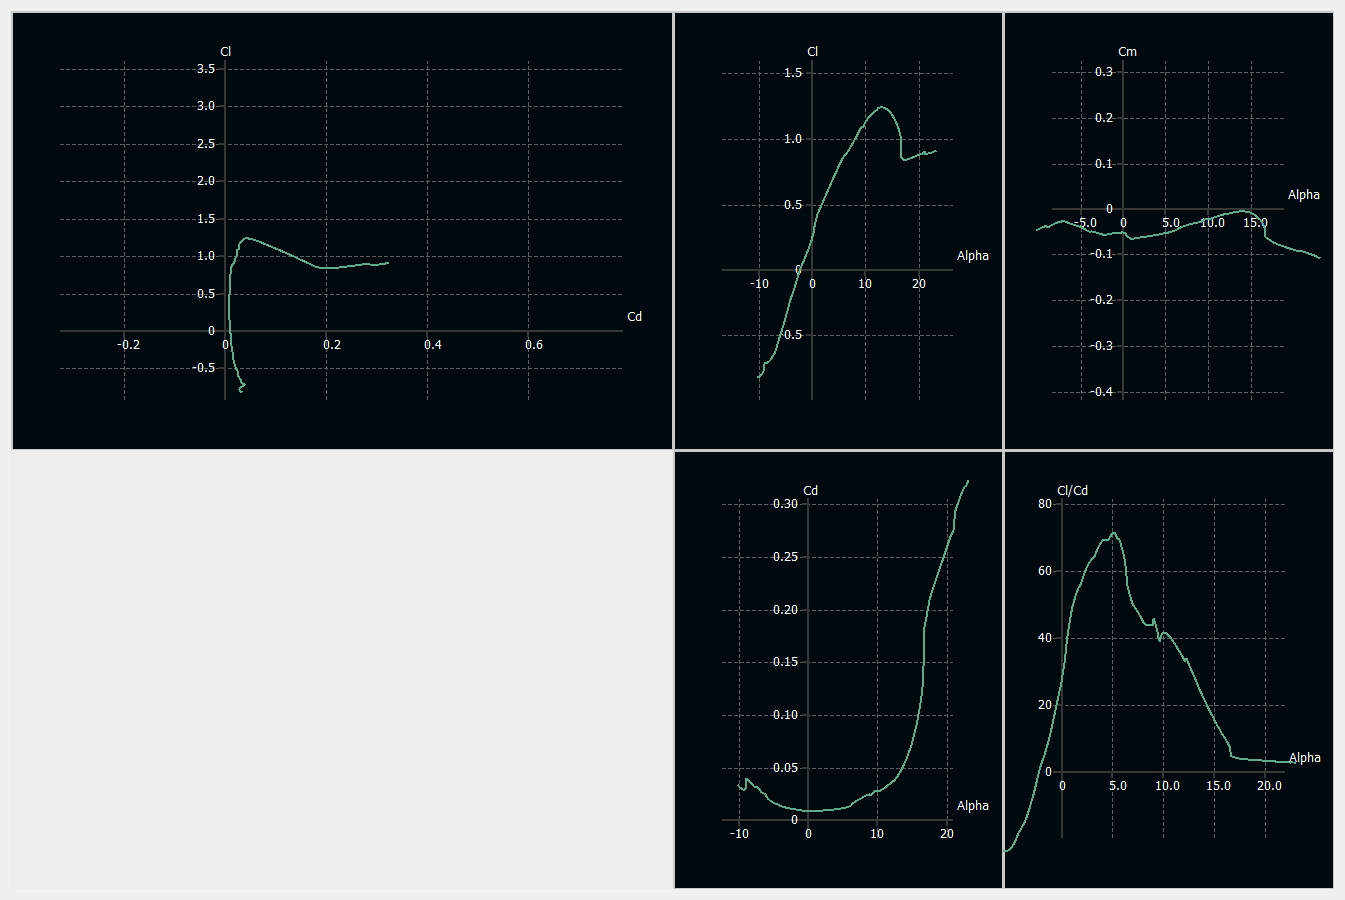
\includegraphics[width=\textwidth]{naca2412-aa1.png}
        \caption{Airfoil analysis - 1}
        \label{fig:naca-2412-aa1}
    \end{subfigure}
    \caption{NACA-2412 Airfoil}
\end{figure}

We first analyze the airfoil in \href{https://www.xflr5.tech/xflr5.htm}{XFLR5}, using \texttt{XFoil Direct Analysis}. The Reynold's number is calculated using

\begin{equation}
    R_e = \frac{\bar{c} V_a \rho}{\mu} = \frac{0.2 \times 20 \times 1.184}{1.849\times 10^{-5}} = 256138.45 \approx 256140  
\end{equation}

The first analysis is shown in figure \ref{fig:naca-2412-aa1}.

We notice that highest $\sfrac{C_l}{C_d}$ occurs at $\alpha = 5^\circ$ (best lift and least drag). The lift peaks at $\alpha=13^\circ$, with the drag elbowing and then increasing rapidly afterwards. This means that for this airfoil, the preferred angle of attack in the 3D plane design should be from $5^\circ$ to $13^\circ$.

Noting these observations, we proceed with selecting the \texttt{NACA 2412} airfoil.

\subsubsection*{Wing Design - Phase 2: Wing from airfoil}

Running an \texttt{LTT} analysis on a \emph{wing only} model of a plane (using the wingspan $b = 1.1$ and chord $\bar{c} = c = 0.2$) yields figure \ref{fig:wing-phase1}.

\begin{figure}[ht]
    \centering
    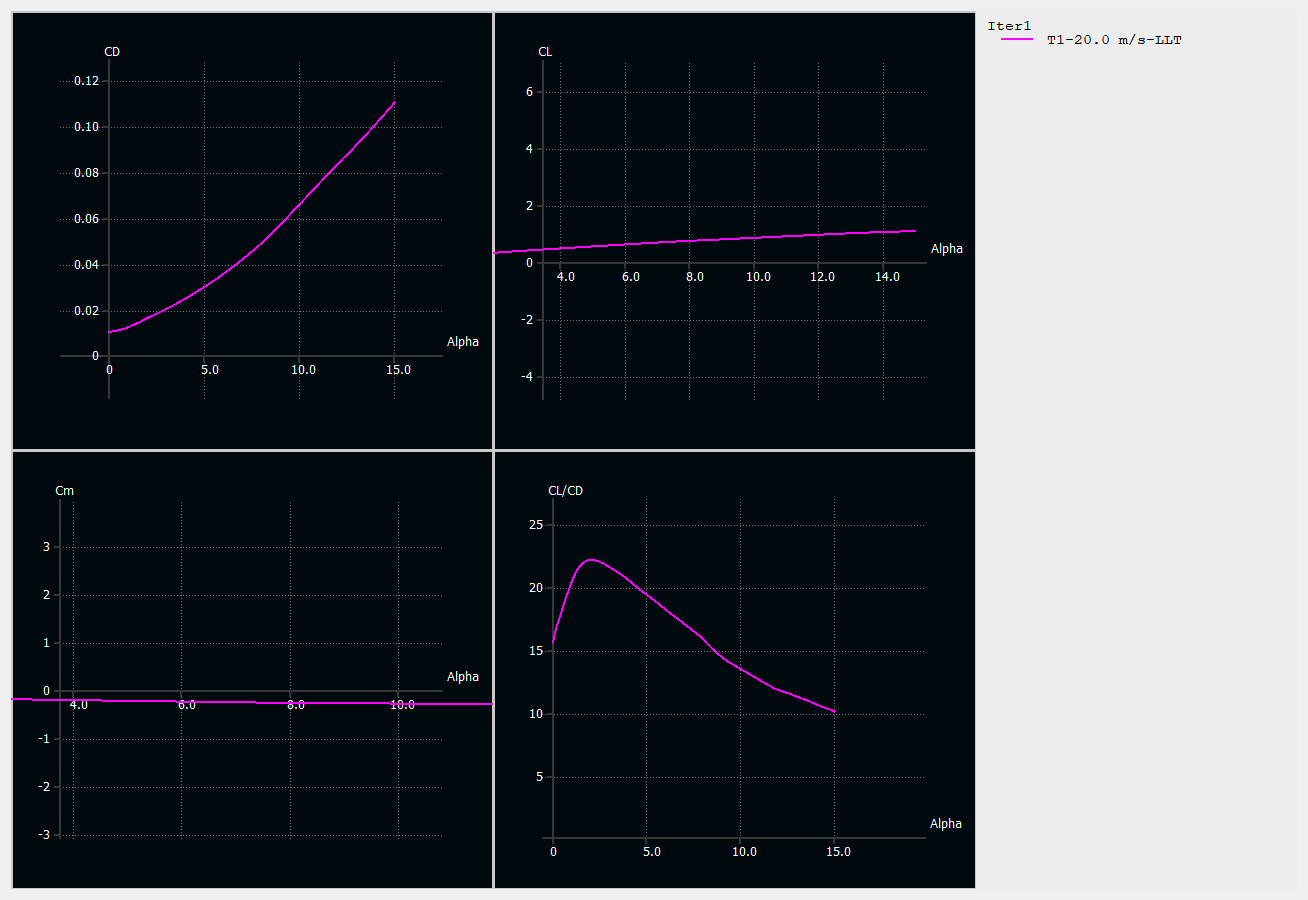
\includegraphics[width=0.5\textwidth]{wing-phase1.png}
    \caption{Wing analysis}
    \label{fig:wing-phase1}
\end{figure}

Fitting the line and quadratic equations through graphs in figure \ref{fig:wing-phase1}, we get

\begin{align}
    C_{L_w} = 3.2944 \alpha + 0.2951 &&
    C_{M_w} = -0.5991 \alpha - 0.1522 &&
    C_{D_w} = 0.7666 \alpha^2 + 0.2022 \alpha + 0.0065
\end{align}

We need to counter the weight for lift (when cruising at steady state). This gives us

\begin{equation}
    F_{L_w} = C_{L_w} \, \frac{1}{2} \rho V_a^2 S_w
    \Rightarrow C_{L_w} = \frac{mg}{\frac{1}{2} \rho V_a^2 S_w}
\end{equation}

We get $C_{L_w} = 0.37622$ for $V_a = 20$, giving us $\alpha = 1.4^\circ$. We can probably fly the plane with this $\alpha$ as well, as seen in figure \ref{fig:naca-2412-aa1}.

If we want the \emph{most} optimal performance for the airfoil (highest $\sfrac{C_l}{C_d}$), we should choose to fly at around $16\,m/s$ (cruise). However, highest $\sfrac{C_L}{C_D}$ is found at around $\alpha = 2.1^\circ$. Our $V_a = 20\,m/s$ should be manageable.

\paragraph*{Tail Design - Phase 3: Horizontal Tail}

We place the tail such that at cruise speed, the pitching moment (along Y axis) is zero. The moment should be negative when $\alpha$ of wing increases, and should be positive when $\alpha$ of wing decreases from the cruise value. This will make the plane self stabilizing.

Through XFLR experimentation, we find that keeping $c = 0.2$, $b = 0.15$ for the horizontal tail is ideal (shape-wise). We place the tail $0.7\,m$ behind the wing, at a tilt of $-5^\circ$. This is shown in figure \ref{fig:sfig-wing-htail}.

\begin{figure}[ht]
    \centering
    \begin{subfigure}[b]{0.4\textwidth}
        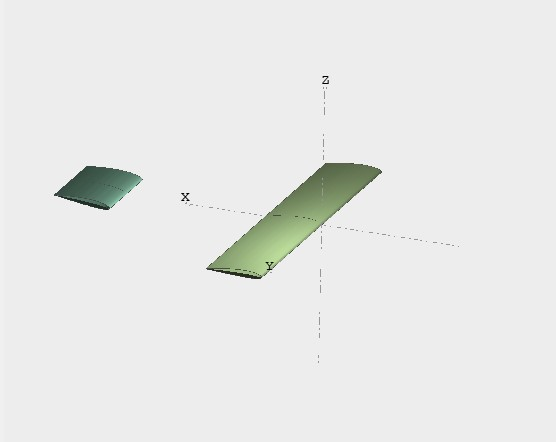
\includegraphics[width=\textwidth]{plane-with-htail.jpg}
        \caption{Horizontal tail}
        \label{fig:sfig-wing-htail}
    \end{subfigure}
    \begin{subfigure}[b]{0.4\textwidth}
        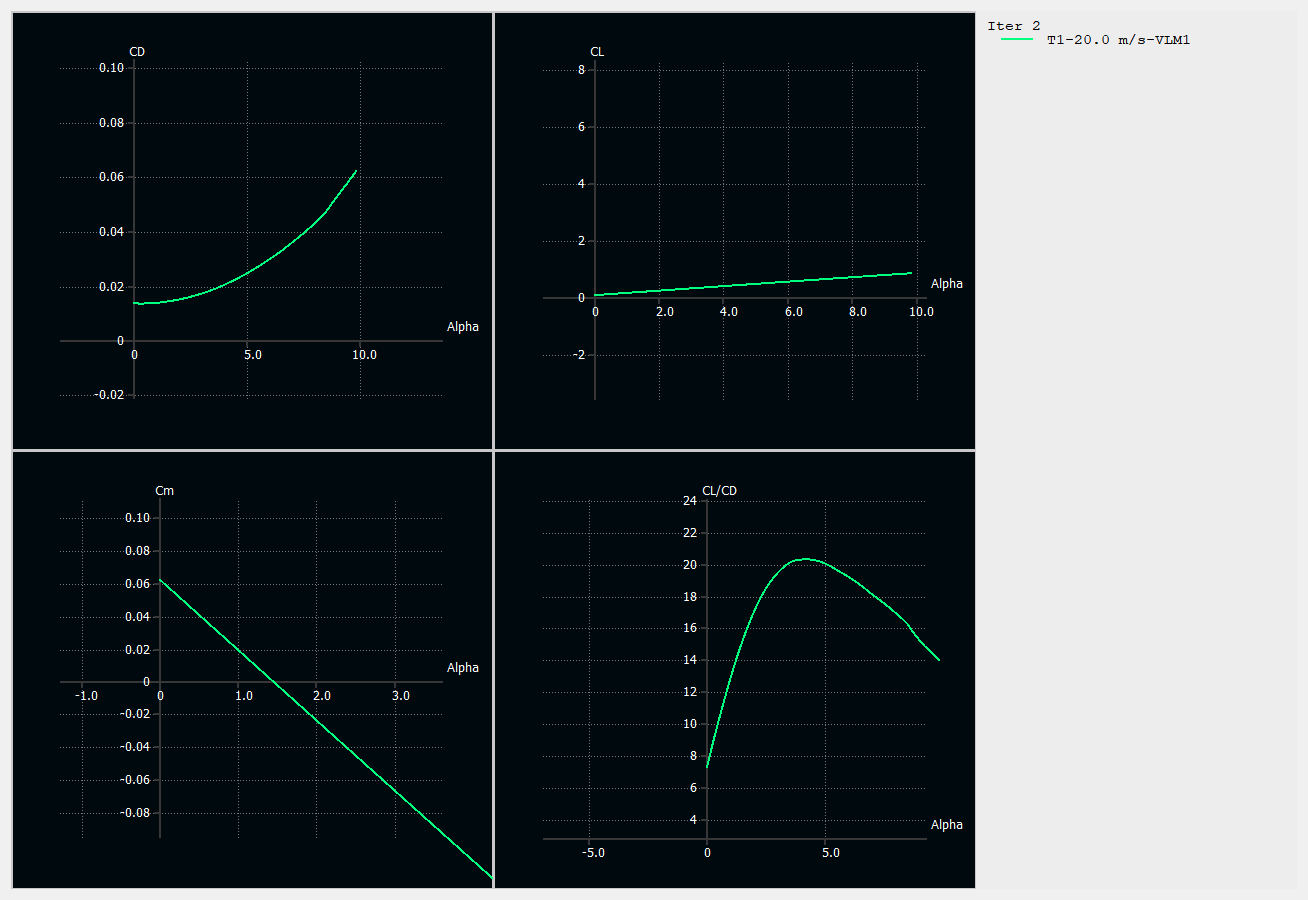
\includegraphics[width=\textwidth]{wing-htail-phase2.png}
        \caption{XFLR Analysis}
        \label{fig:sfig-phase2-xflr}
    \end{subfigure}
    \caption{Wing with Horizontal tail}
\end{figure}

As is visible in the bottom left graph of figure \ref{sub@fig:sfig-phase2-xflr}, the moment counters change in $\alpha$ and will make the plane passively stable. Minor adjustments can be done through control surface designing (elevator).

\subsubsection*{Tail Design - Phase 4: Vertical Tail}

This needn't be too complicated, we don't need to make agile maneuvers. We can choose an airfoil with zero camber so that it passively doesn't add yaw, something like \texttt{NACA 0012} airfoil should work.

We run a batch analysis with a range of Reynolds number for \texttt{NACA 0012} and end up with the results in figure \ref{fig:sfig-naca0012-ba}.

\begin{figure}[ht]
    \centering
    \begin{subfigure}[b]{0.3\textwidth}
        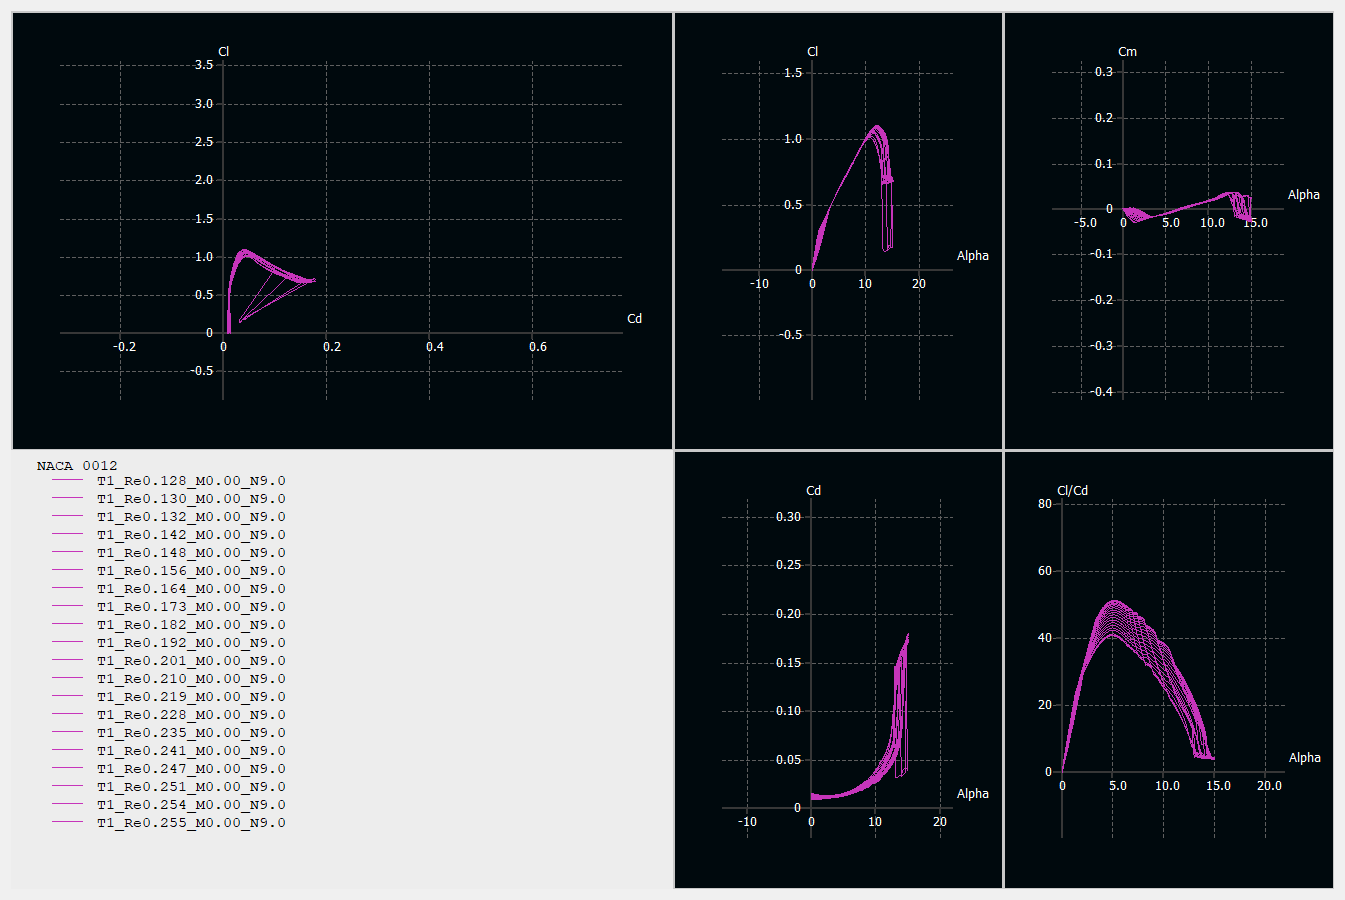
\includegraphics[width=\textwidth]{naca0012-ba1.png}
        \caption{NACA 0012}
        \label{fig:sfig-naca0012-ba}
    \end{subfigure}
    \begin{subfigure}[b]{0.3\textwidth}
        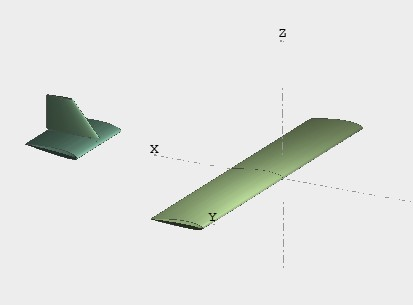
\includegraphics[width=\textwidth]{plane-with-vtail.jpg}
        \caption{Final plane}
        \label{fig:sfig-plane-vtail}
    \end{subfigure}
    \begin{subfigure}[b]{0.3\textwidth}
        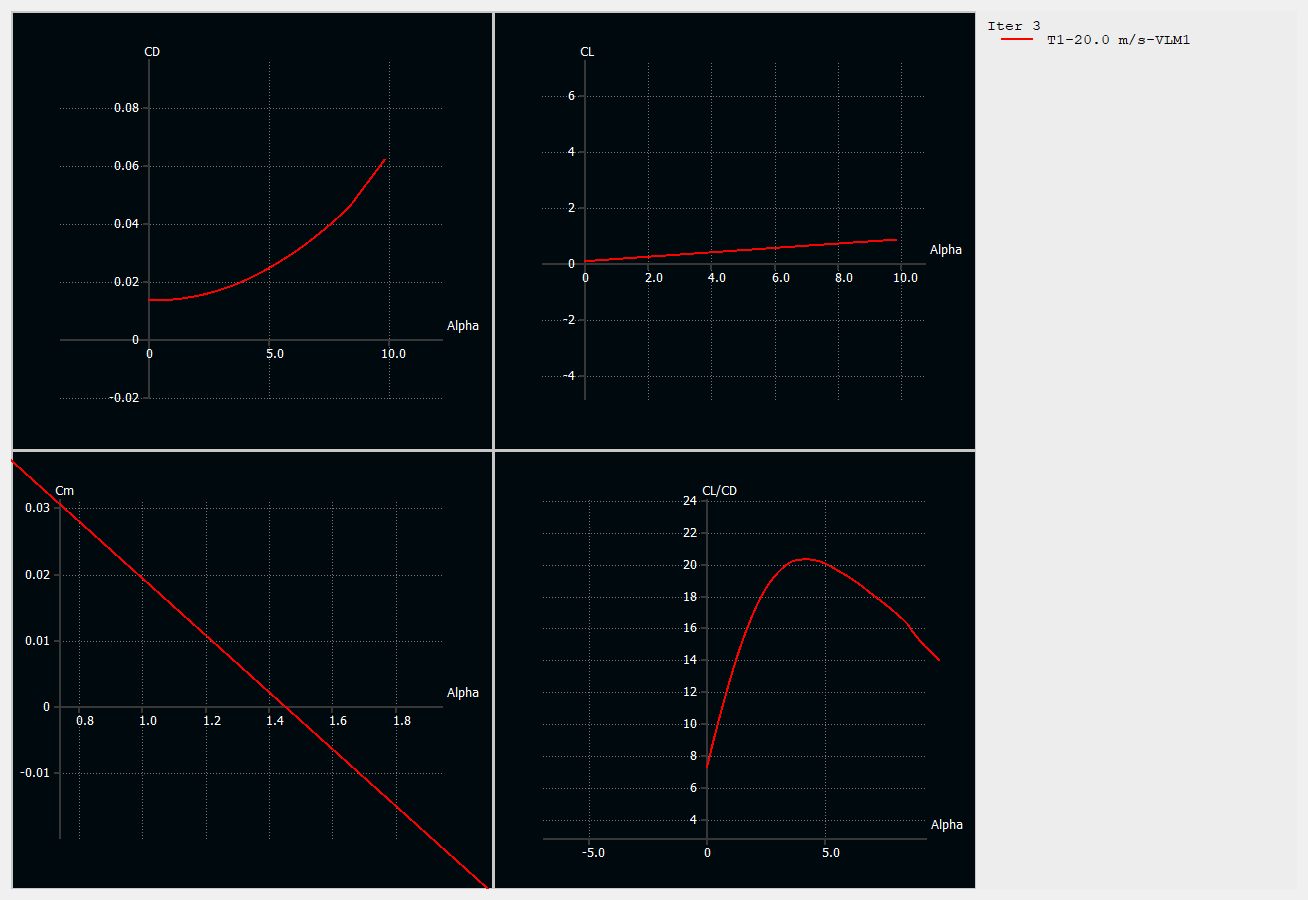
\includegraphics[width=\textwidth]{wing-vtail-phase3.png}
        \caption{XFLR Analysis}
        \label{fig:sfig-vtail-analysis}
    \end{subfigure}
    \caption{Final plane design}
    \small
        NACA 0012 airfoil for the vertical tail. The plane analysis is presented here.
\end{figure}

We then attach the vertical tail at $0.7\,m$ X and $0.025\,m$ Z, with \texttt{NACA 0012} airfoil and taking chord $0.20$ at base and $0.10$ at the top ($0.120$ height).
The final plane is visible in figure \ref{fig:sfig-plane-vtail}.

After running analysis on the plane (we do not expect much change from previous phase), we get figure \ref{fig:sfig-vtail-analysis}.

\subsubsection*{Control Surface}

The \textbf{elevator} and \textbf{rudder} are chosen at $35\%$ and $25\%$ of the chord length of horizontal and vertical tail respectively.

Based on historical data, we choose the \textbf{aileron} to span $37.5\%$ of the wing, while spanning $25\%$ of the chord.

\subsubsection*{Conclusion Notes}

\begin{itemize}
    \item We could have chosen a \emph{sweepback} wing planform instead of a \emph{rectangular} one. This will require a detailed batch analysis for the \texttt{NACA 2412} airfoil, as well as a more detailed review of the pitch and yaw control (as there will be no need of a tail). This will save a lot of space, but will make the design process more complicated (hence not attempted here).
    \item The horizontal tail could also be a zero camber one, but with a different tile angle. We went with choosing the same airfoil as the wing.
    \item We can add $10\%$ wing tips at both sides of the wing to prevent vortex drag. But this will require some advanced analysis (for new drag and lift calculations).
    \item Sometimes during analysis, we could gett a \texttt{Point out of flight envelop} error (this is because of interpolation issues). Seems like, the best fix is running a detailed batch analysis beforehand \footnote{From \href{https://www.xflr5.tech/docs/Point_Out_Of_Flight_Envelope.pdf}{xflr5.tech/docs/}}.
\end{itemize}
